El marco lógico para abordar la lectura de imágenes constituye en sí mismo una insinuación metodológica. En este sentido, es necesario precisar cómo el montaje, en tanto método, aporta significado a la constelación saturada de tensiones que contienen y manifiestan las imágenes.

El método del montaje, comprende dos acciones fundamentales según \parencite{Guasch2005}: archivar y articular. Este enfoque implica el abandono de los métodos y categorías analíticas formalistas, como se evidencia en los paneles del Atlas Mnemosyne de Aby Warburg, donde la memoria social es interpelada a través de la imagen. Se establece así una sutil pero significativa conexión entre el ejercicio metodológico de Walter Benjamin en \textit{El Libro de los Pasajes} y el \textit{Atlas Mnemosyne} de Warburg, unidos por un método común de construcción de significados: el montaje. \textcolor{edit30sept}{En esta investigación, dichas acciones se integran en una \textit{meta-composición estética y documental}, entendida como la articulación de segundo orden que reescribe el archivo en escenas, habilitando una lectura reflexiva del \textit{síntoma} y el \textit{anacronismo} como operadores de sentido.}

Los paneles que Warburg construyó en 1925 constituyen conjuntos de imágenes heterogéneas que incluyen fotografías, reproducciones de grabados, miniaturas, recortes publicitarios, mapas y sellos. Estos 79 paneles, dispuestos en una aparente disposición caótica, representan un modelo particular de archivo y construcción de sentido basado en la discontinuidad y heterogeneidad de las imágenes.

Como señala \parencite{Guasch2011}, el Atlas de Warburg emerge como un proyecto archivístico e icónico que desafía deliberadamente los límites restrictivos de la historia del arte tradicional, caracterizada por sus compartimentaciones jerárquicas, abandonando así los métodos y categorías analíticas exclusivamente formalistas o estilísticas.

Como señala \parencite{Guasch2005}, "el archivo, tanto desde un punto de vista literal como metafórico, se entiende como el lugar legitimador para la historia cultural. Como afirma el filósofo Michel Foucault, el archivo es el sistema de «enunciabilidad» a través del cual la cultura se pronuncia sobre el pasado" (p. 157). Esta perspectiva nos permite navegar el entramado de imágenes emergentes, originarias, turbulentas, entrecortadas y sintomáticas del fenómeno de crisis.

\textcolor{edit30sept}{\parencite{Guasch2011} propone una lectura cruzada entre Warburg y Benjamin. Warburg, pionero de la iconología y del método de montaje visual, desarrolló una metodología histórica fundamentada en tres ejes principales}, como se señala en \parencite{Warburg2010}: "la relación entre textos e imágenes, su idea de encontrar la huella de la antigüedad en el movimiento patético de figuras, ropajes y otros elementos accesorios, y la fundamentación psicológica de sus estudios en la teoría de la empatía" (p. 135). Por su parte, Benjamin aporta la noción antipositivista de historia e "historia a contrapelo", dedicando especial atención al modelo epistemológico del Atlas Mnemosyne de Warburg.


\parencite{DidiHuberman2011} argumenta que la colisión temporal en la imagen libera todas las modalidades del tiempo mismo, desarrollando una paradójica noción donde, aunque la imagen se dispersa en la historia, también se cristaliza en obras específicas. Las imágenes contienen frágiles supervivencias que provocan emociones y comprensión no-verbal. Al desmontar el registro de obra plástica, documental, fotográfica, dramatúrgica o performativa de su función y contexto original, se revelan aspectos del fenómeno que trascienden los motivos iconográficos o mensajes iconológicos tradicionales, generando un conocimiento a través del montaje.

El montaje, según \parencite{DidiHuberman2011}, emerge como una operación fundamental del conocimiento histórico, caracterizando simultáneamente el objeto de este conocimiento: el historiador recopila los "desechos" porque estos poseen la doble capacidad de desmontar la historia y montar el conjunto de tiempos heterogéneos, conectando el Tiempo Pasado con el Ahora, la supervivencia con el síntoma, la latencia con la crisis. \textcolor{edit30sept}{Esta doble capacidad del montaje se formaliza aquí como \textit{meta-composición}, donde los ‘desechos’ y discontinuidades del archivo constituyen unidades plásticas de recomposición escénica.}


\begin{figure}[ht]
    \centering
    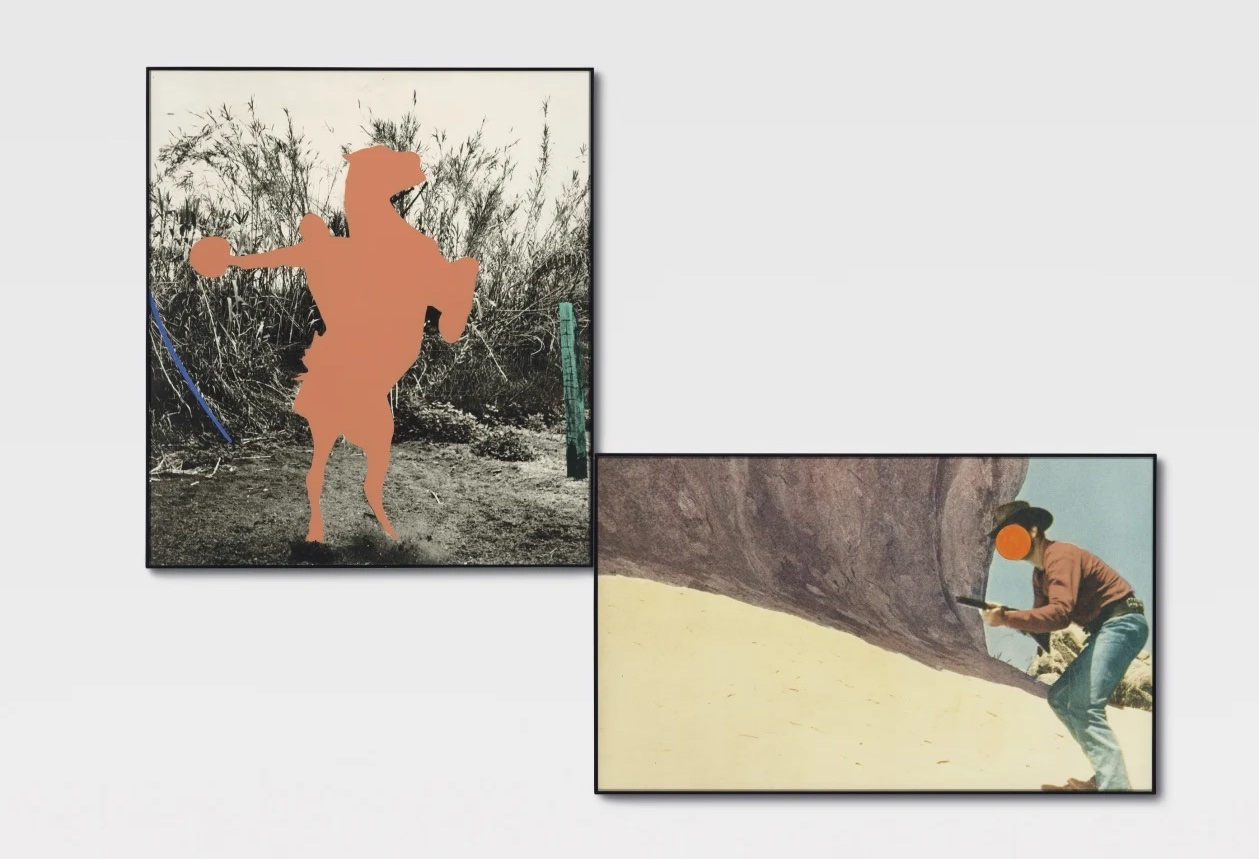
\includegraphics[width=\textwidth]{pulpogallery-john-baldessari-equestrian-flesh-1992.jpg}
    \caption{John Baldessari, \textit{Equestrian (Flesh) in Brackets with Orange Showdown}, 1992.}
    \label{fig:baldessari_equestrian}
\end{figure}


La obra \textit{Equestrian (Flesh) in Brackets with Orange Showdown} de John Baldessari ejemplifica el uso de la imagen-archivo como estrategia de producción artística\footnote{En el libro \textit{Arte y archivo, 1920-2010. Genealogías, tipologías y discontinuidades de Anna María Guasch} la autora dedica tudo un acápite titulado \textit{John Baldessari: el archivo como montaje} a explicar el  particular método de construcción de sentido visual empleado por Bassari mediante el montaje y decomposición lineal.}. Esta práctica, característica de su enfoque conceptual, se fundamenta en la apropiación y recontextualización de material visual preexistente. El artista no genera las fotografías originales, sino que las selecciona meticulosamente de archivos contemporáneos, incluyendo fotogramas cinematográficos hollywoodenses y otros materiales visuales de la cultura popular. Mediante intervenciones con pintura acrílica, Baldessari transforma el significado original de estas imágenes, generando nuevas capas de sentido que exploran cuestiones fundamentales sobre identidad, percepción y narrativa visual.

\begin{quote}
    El interés de Baldessari no se dirige, pues, a la historia en sí misma, sino a <<cómo contar la historia>> a través de la selección y combinación de imágenes. Al eliminar la narración lineal, deja que las diferencias de los elementos operen como un nudo de vías de comunicación a través del cual se posibilita un orden variable. Es precisamente la disposición sincrónica de las imágenes lo que permite que estas puedan finalmente ser leídas y releídas según múltiples direcciones.\parencite[p. 113-114]{Guasch2011}
\end{quote}

Estos "desechos" representan cristalizaciones modestas de la existencia, impurezas que se filtran entre las grietas y recovecos del fenómeno observado. En estas impurezas persiste el pasado, permitiéndonos manipular los hilos del tiempo y construir nuevas narrativas históricas.

 
\begin{figure}[ht]
    \centering
    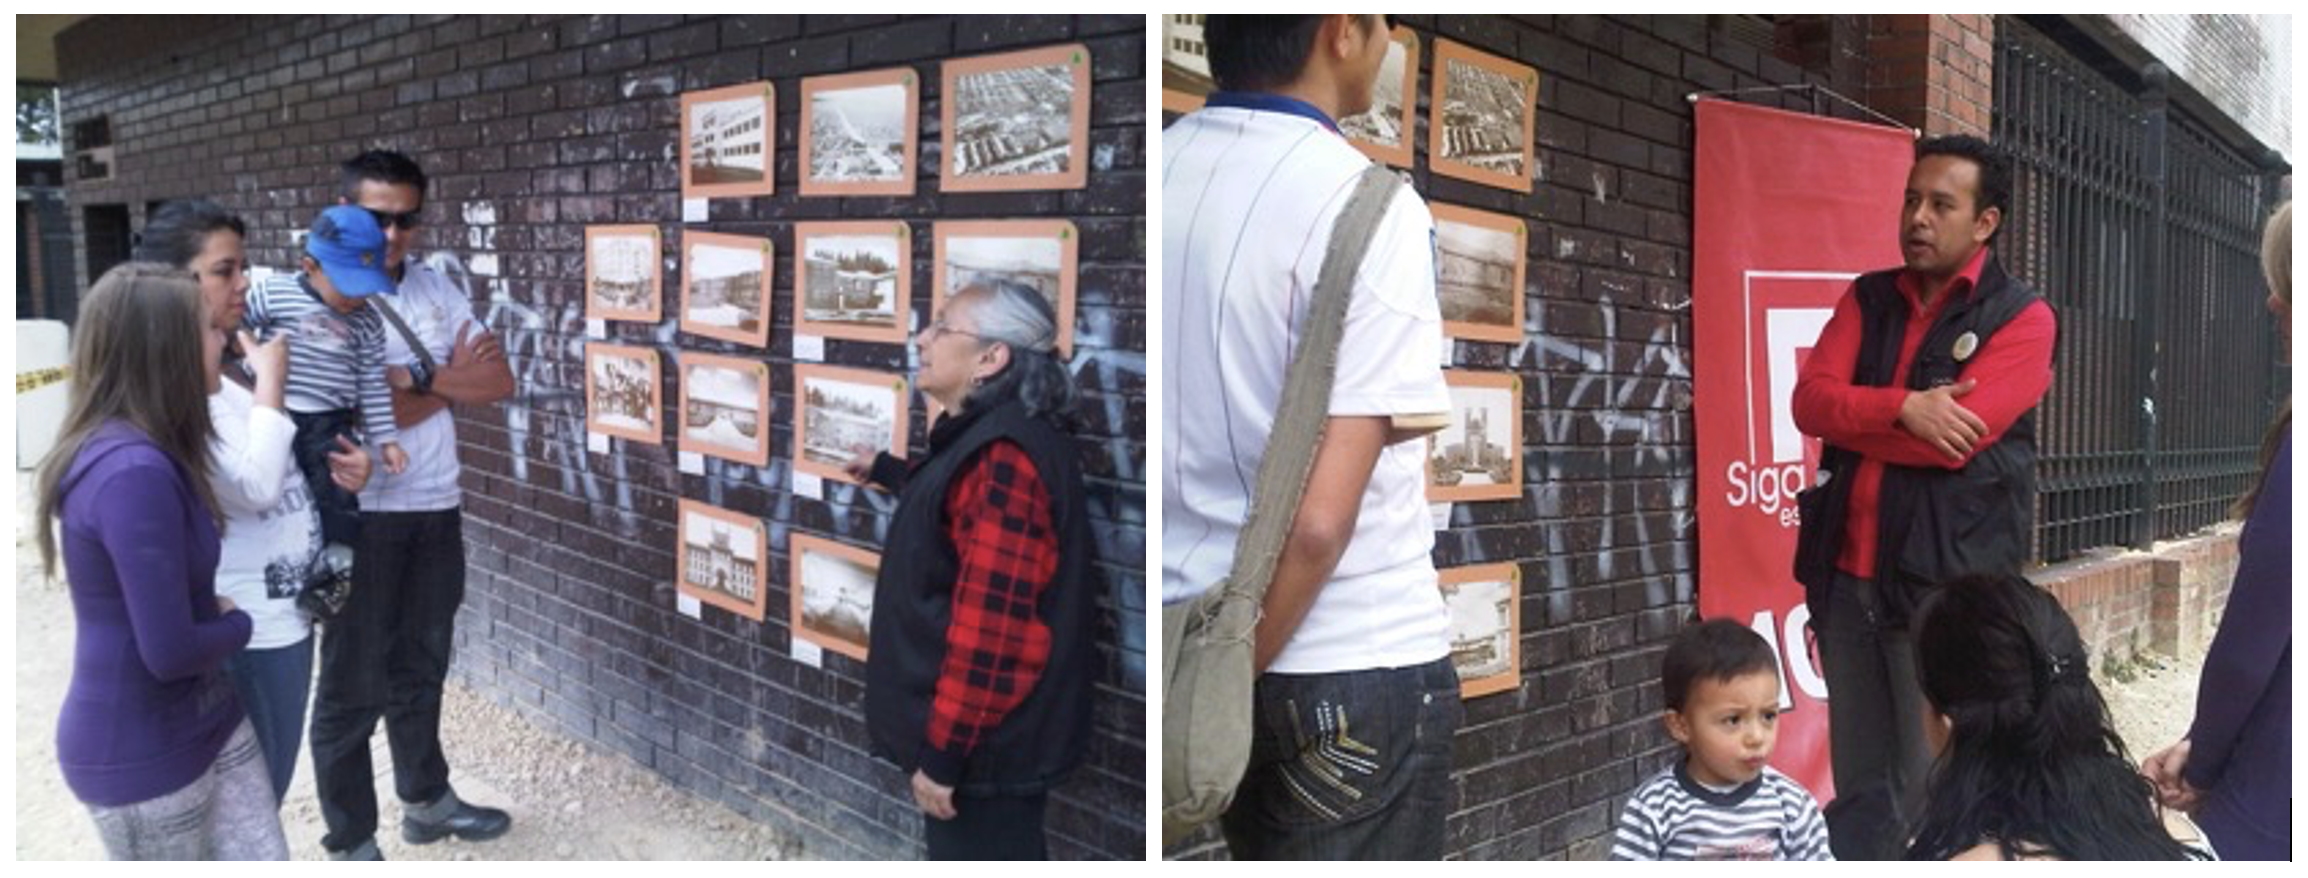
\includegraphics[width=\textwidth]{siga-esta-es-su-casa.png}
    \caption{Estación recorrido ``Siga esta es su casa'' (2008). Foto Archivo Margarita Castro}
    \end{figure}
    
La práctica de comprender el caso del Hospital San Juan de Dios a través de imágenes se estableció mucho antes que las experiencias de la mirada artística. En la Figura 1 se observan dos momentos de la visita "Siga esta es su casa", una de las estaciones de estos recorridos que originalmente se realizaban de forma autónoma como resistencia al olvido \parencite{Gongora2013}. Estos recorridos, inicialmente prohibidos durante el proceso de liquidación de la entidad, han resurgido después de muchos años. Sus promotores principales, la enfermera Margarita Castro y el arquitecto David Cristancho, son memoria viva que al guiar estos recorridos por el complejo hospitalario lo "actúan", manteniendo la estructura original. Durante 2022, esta práctica se transformó en una puesta en escena, desarrollándose en paralelo a otras acciones performativas y memoriales, como parte de un esfuerzo conjunto entre el Ministerio de Cultura, la Gobernación de Cundinamarca, el Instituto Distrital de Patrimonio Cultural (IDPC) y la Secretaría Distrital de Salud, para la intervención integral de siete de los diecisiete edificios de mayor valor patrimonial del Complejo Hospitalario \parencite{IDPCSanJuanDeDios}.
    
\begin{figure}[ht]
    \centering
    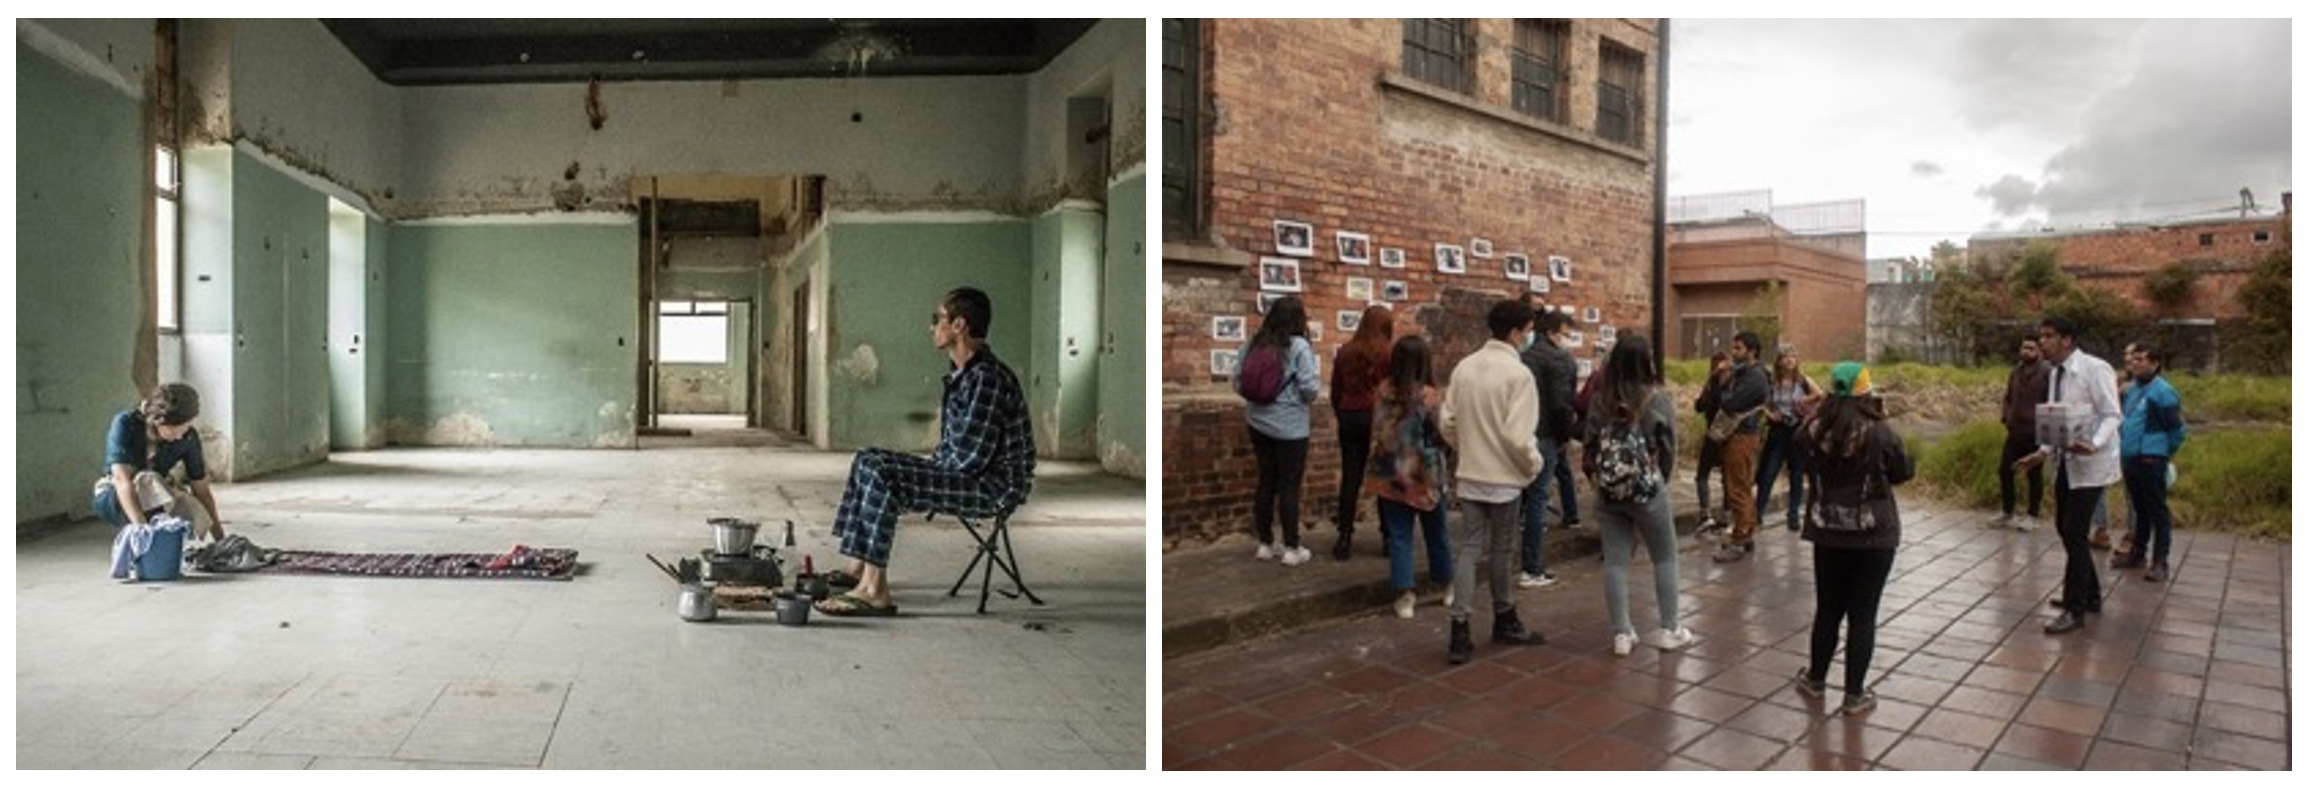
\includegraphics[width=\textwidth]{recorridos-idpc.png}
    \caption{Recorridos patrimoniales IDPC (2022). Foto: Juan Carlos Arroyo.}
\end{figure}

La Figura 3.3 muestra dos momentos de los recorridos patrimoniales coordinados por el IDPC. Estas prácticas performativas de sensibilización \parencite{Guasch2011} incluían la ilustración de momentos históricos mediante imágenes montadas sobre los muros exteriores del hospital. Cada imagen, impresa sobre papel, llevaba pequeñas notas históricas, replicando el formato de los recorridos originales del "Siga esta es su casa" realizados más de una década antes.

Resulta notable la capacidad del complejo hospitalario para convocar distintos actos de ver \parencite{Abril2007}, ya sean ejercicios de resistencia social, prácticas de memoria, acciones patrimoniales o, como ha ocurrido en varias ocasiones, escenario para la exhibición de obras de arte, relacionadas o no con el fenómeno de crisis del HSJD.

\begin{figure}[ht]
    \centering
    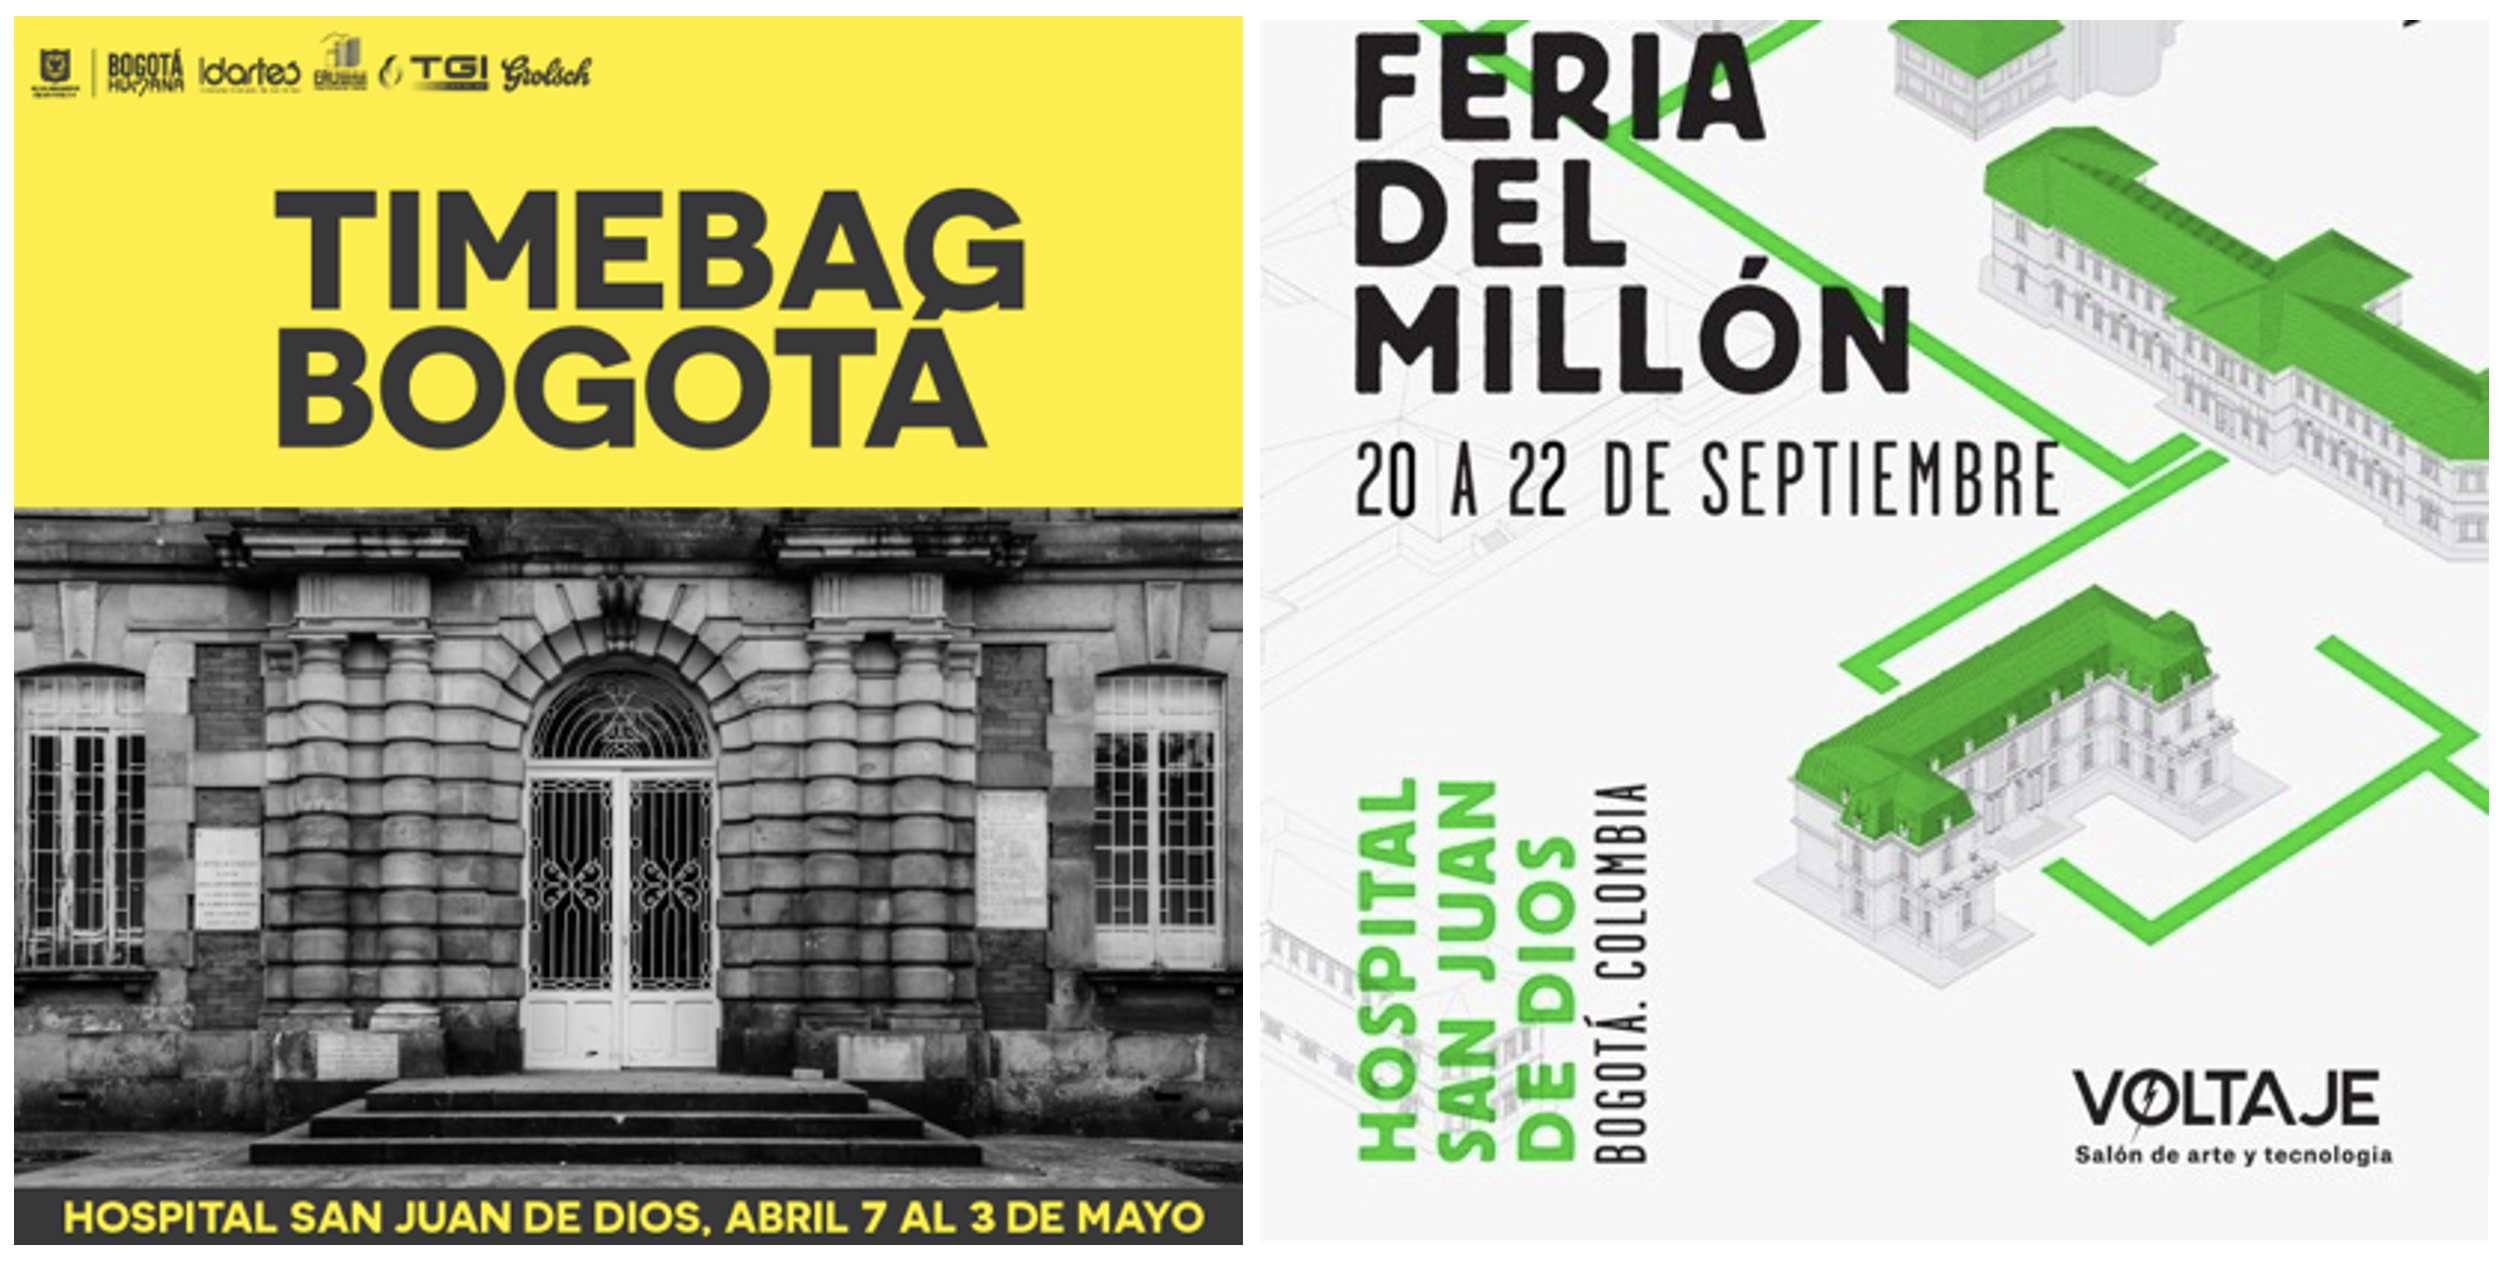
\includegraphics[width=\textwidth]{carteles.png}
    \caption{Carteles publicitarios TimeBag y Feria del Millón.}
\end{figure}

Dos eventos significativos fueron \textit{TimeBag Bogotá} y \textit{La Feria del Millón}, donde se evidenció la similitud en la práctica del montaje que, independiente de su intención, replica la práctica expositiva inherente al HSJD. Estos eventos crearon espacios de enunciación discursiva no-textual que, por desarrollarse dentro de este poderoso escenario patrimonial y simbólico, contribuyeron durante su efímera existencia al imaginario social sobre la crisis del San Juan.

El Hospital San Juan de Dios ha servido como escenario de montaje para prácticas memoriales, artísticas y performativas que, independientemente de su sensibilidad frente al fenómeno de crisis, generan imágenes de registro que se integran a la red significante e imaginaria, dada su escenificación reconocible al interior del complejo arquitectónico \parencite{BuckMorss1989}.

\begin{figure}[ht]
    % Nota: El nombre del archivo tenía la ó en forma descompuesta (o + \' ) causando error en algunos sistemas.
    % Se reemplaza por la versión NFC directa "ó" para que coincida con el archivo en disco.
    \includegraphics[width=\textwidth]{Pabellón San Lucas.png}
    \caption{Pabellón San Lucas (2001 y 2019). Archivo: IDPC.}
\end{figure}

\subsection*{El montaje}

La selección de imágenes constituye el primer paso fundamental en la construcción de sentido. Este proceso selectivo nos permite explorar la memoria social y nuestro inconsciente, revelando aspectos que normalmente permanecen ocultos tras la aparente cotidianidad de las imágenes.

El \textit{corpus} de análisis, abordado mediante el método del montaje, comprende una colección de registros de obras de arte y activaciones culturales y memoriales realizadas en el Hospital San Juan de Dios (HSJD) entre 2000 y 2015. Adicionalmente, se incluyen imágenes significativas del año 2022 relacionadas con nuevas activaciones en torno al patrimonio.

Esta colección resulta particularmente reveladora por presentar imágenes que trascienden la cotidianidad operativa de un hospital. No se trata de reportería gráfica ni de imágenes inocentes; los registros artísticos y culturales materializan visualmente el San Juan como imágenes dialécticas, cargadas de deseos y potencial imaginativo. Como señala \parencite{DidiHuberman2011}: "Las imágenes dialécticas son símbolos de deseo (Wunsche). En ellas se presentan, al mismo tiempo que la cosa misma, el origen (Ursprung) y la decadencia (Untergang) de éste" (p. 169).

Durante el período activo de producción visual sobre el HSJD convergieron diversos intereses y formas de participación: artísticas, filosóficas, historicistas, antropológicas, de gestión cultural y agenciamiento social, memorial y comunitario.

Los registros visuales de estas intervenciones -sean obras plásticas, documentales, fotografías, dramaturgias o performances- han generado un repertorio de «memoria visual» que, en conjunto, enriquece la interpretación del fenómeno. Como señala \parencite{Abril2007}, esta construcción de sentido puede prescindir de la mediación textual o el ordenamiento cronológico, permitiendo que emerja la categoría benjaminiana de «imagen dialéctica», donde pasado y presente "destellan en una constelación" (p. 109).

La selección no pretende representar cronológicamente acontecimientos relevantes del HSJD, sino reunir diversas manifestaciones discursivas de resistencia sobre su crisis y cierre. Busca comprender tanto la emergencia de estas imágenes como sus contenidos en relación con el entorno vital y cultural de la crisis institucional.

El corpus de estudio comprende registros de obras plásticas, audiovisuales, fotográficas e instalaciones, junto con imágenes de archivos personales de los entrevistados. Estos objetos visuales serán "montados" en escenas para construir sentido mediante imágenes-síntoma y anacronismos.

\textcolor{edit30sept}{Los criterios de selección se fundamentan en la identificación de elementos en la imagen que sean suceptibles de poner en juego la mirada del espectador, privilegiando imágenes-síntoma y anacronismos que revelan tensiones interpretativas. El montaje, siguiendo el método warburguiano, explora conexiones dialécticas entre memoria histórica, supervivencias culturales y manifestaciones sintomáticas del fenómeno de crisis.}

Como señala \parencite{Benjamin2004}, el montaje interrumpe el contexto establecido, forzando tanto al espectador como al actor a tomar postura ante los sucesos presentados. Esta interrupción no busca estimular, sino organizar la experiencia visual (p. 52).

Las obras artísticas, archivos fotográficos y dramatúrgicos seleccionados funcionan como memoria social, escenificando acontecimientos históricos y sociales que aluden a relaciones complejas, sin necesidad de responder a jerarquías, sistemas lógicos o narrativas lineales.

La metodología de análisis de imagen se fundamenta en dos marcos de referencia principales: el método de montaje propuesto por Walter Benjamin \parencite{BuckMorss1989} y el M12 desarrollado por Rubén Dittus \parencite{Aliaga2022}. Este proceso metodológico se estructura en dos fases, así:

\textcolor{edit30sept}{En el contexto contemporáneo de análisis visual, las herramientas de inteligencia artificial han comenzado a complementar los métodos tradicionales de catalogación y descripción de imágenes. En particular, OpenAI GPT-4 Vision representa una tecnología capaz de analizar, interpretar y etiquetar imágenes de manera automatizada mediante redes neuronales profundas entrenadas con extensos corpus visuales. Esta tecnología permite reconocer objetos, escenas, expresiones y contextos visuales complejos, generando descripciones precisas que facilitan la organización sistemática del material visual y enriquecen la interpretación crítica a partir del reconocimiento automático de patrones e imaginarios presentes en las imágenes. Si bien estas herramientas digitales proporcionan un apoyo técnico valioso para la sistematización inicial del \textit{corpus} visual.}
\section{Selección}

a) \textbf{Elección de las imágenes:} La selección del corpus discursivo se constituye a partir de imágenes artísticas que abordan o se contextualizan en la crisis del Hospital San Juan de Dios de Bogotá. Este proceso implica una cuidadosa identificación y catalogación de obras que documentan visualmente este período histórico.

b) \textbf{Caracterización de manifestaciones del discurso:} El análisis comprende textos visuales que evidencian una corporeidad inequívoca del objeto de estudio. Este corpus integra registros de obras artísticas, material fotográfico y literatura generadora de imágenes mentales, todos ellos vinculados explícitamente con el fenómeno de crisis y cierre del Hospital San Juan de Dios. La selección prioriza aquellas manifestaciones que aportan significativamente a la construcción de la memoria colectiva del hospital.

c) \textbf{Descripción de la estructura:} El análisis de la estructura dialógica en los textos visuales seleccionados requiere la identificación sistemática de escenas que agrupan símbolos, signos denotativos, anacronismos e imágenes-síntoma. Este proceso analítico se fundamenta en los conceptos de la antropología de las imágenes y la sociosemiótica \parencite{Abril2007}, permitiendo una comprensión profunda de las capas de significado presentes en cada representación visual.

\section{Montaje}

a) \textbf{Escenarios para imaginarios:} El proceso interpretativo emerge desde la perspectiva del intérprete-espectador, estableciendo un diálogo dinámico entre la mirada y la imagen. El imaginario social que sustenta este dialogismo se fundamenta en la cultura visual contemporánea y la concepción colectiva del hospital: su pasado, su ideal y las transformaciones del imaginario social del HSJD provocadas por la crisis y el cierre \parencite{Gongora2013}. Esta aproximación permite comprender cómo las representaciones visuales contribuyen a la construcción de la memoria colectiva.

b) \textbf{Red significante:} El discurso seleccionado se articula en torno a conceptos totalizadores fundamentales: la salud pública, el cuidado humano y el imaginario del HSJD ideal. La crisis y el posterior cierre evidencian desequilibrios críticos en la operatividad hospitalaria, afectando no solo la prestación general de servicios de salud pública, sino también el cuidado humano, las historias de vida y la preservación de sujetos históricos y patrimoniales. Esta red de significados permite comprender la complejidad del impacto social y cultural de la crisis hospitalaria.

